\documentclass[
]{jss}

\usepackage[utf8]{inputenc}

\providecommand{\tightlist}{%
  \setlength{\itemsep}{0pt}\setlength{\parskip}{0pt}}

\author{
Hanne Oberman\\Utrecht University \And Johanna Munoz Avila\\University
Medical Center Utrecht \AND Valentijn de Jong\\University Medical
Center Utrecht \And Gerko Vink\\Utrecht University \AND Thomas
Debray\\University Medical Center Utrecht
}
\title{Imputation of Incomplete Multilevel Data with \pkg{mice}}

\Plainauthor{Hanne Oberman, Johanna Munoz Avila, Valentijn de
Jong, Gerko Vink, Thomas Debray}
\Plaintitle{Imputation of Incomplete Multilevel Data with mice}
\Shorttitle{\pkg{mice}: Multilevel}


\Abstract{
Tutorial paper on imputing incomplete multilevel data with \pkg{mice}.
Including methods for ignorable and non-ignorable missingness.
}

\Keywords{missing
data, multilevel, clustering, \pkg{mice}, \proglang{R}}
\Plainkeywords{missing data, multilevel, clustering, mice, R}

%% publication information
%% \Volume{50}
%% \Issue{9}
%% \Month{June}
%% \Year{2012}
%% \Submitdate{}
%% \Acceptdate{2012-06-04}

\Address{
    Hanne Oberman\\
    Utrecht University\\
    Padualaan 14\\
3584 CH Utrecht\\
  E-mail: \email{h.i.oberman@uu.nl}\\
  URL: \url{https://hanneoberman.github.io/}\\~\\
          }

% Pandoc syntax highlighting

% Pandoc citation processing


\usepackage{amsmath}

\begin{document}

\hypertarget{introduction}{%
\section{Introduction}\label{introduction}}

\hypertarget{multilevel-data}{%
\subsection{Multilevel data}\label{multilevel-data}}

We talk of multilevel data when there is some kind of hierarchy or
clustering in a dataset. In the typical case, individuals are nested
within groups, but there are many different types of multilevel data. In
the medical field clustering occurs at e.g., the hospitals/center level
in registry data, or at the study-level in meta-analyses (IPDMA). In the
social sciences and official statistics we can find clustering e.g.~at
the country-level, or as imposed by the sampling design. In this paper,
we will refer to the grouping variable as `cluster', and the grouped
variable as `(sample) unit'. For reasons of brevity, we only discuss
clustering between units, not longitudinal data (within-unit
clustering).

Multilevel data requires special care when doing any sort of analysis.
The cluster to which a unit belongs may influence the unit-level
observations, and since clusters are made up of units, clusters depend
on units as well \citep{hox17}. {[}Explain ICC here? The percentage of
variance attributed to the cluster-level is expressed by the intra-class
coefficient (ICC). The ICC can also be interpreted as the expected
correlation between two randomly sampled units in same cluster.{]} These
relations can and should be taken into account when developing analysis
models for multilevel data. At least, such models include a separate
intercept term for each cluster. But there may also be random predictor
effects and/or random error terms (residual error variances), see e.g.
\citet{hox17} and \citet{jong21}. Heterogeneity refers to variability
within clusters vs.~variability between clusters. There are many names
for models that take clustering into account. Some popular examples are
`multilevel models', `hierarchical models', `mixed effect models' and
`random effect models'.

\hypertarget{missing-data}{%
\subsection{Missing data}\label{missing-data}}

\begin{itemize}
\item
  Why/where does missingness occur in multilevel data? I.e., not only
  patient-level but also cluster-level.
\item
  How can we categorize this? Systematic vs sporadic missingness, see
  \citet{resc13}. Within systematic we have two flavors: unobserved
  constants (same value per cluster) and non-measured random variables
  (which may differ per unit within clusters). In figure 1, we show a
  dataset with units in the rows and variables in the columns, there are
  5 units nested within 2 clusters, and 3 variables of interest.
  Variable \texttt{X1} is completely observed. Variable \texttt{X2} is
  systematically missing, \texttt{X3} is sporadically missing. The
  unobserved value for units 4 and 5 on variable \texttt{X2} may be the
  same or different, defining which type of systematic missingness is
  happening.
\end{itemize}

\begin{CodeChunk}


\begin{center}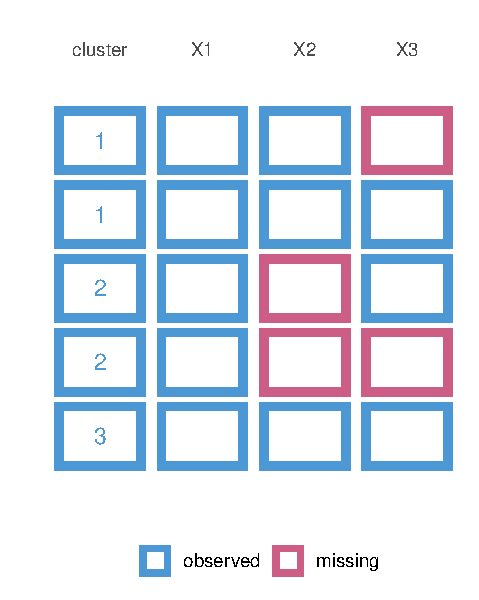
\includegraphics{Manuscript_files/figure-latex/patterns-1} \end{center}

\end{CodeChunk}

\begin{itemize}
\item
  What kinds of missingness are there? ADD: missingness mechanisms here.
  See e.g. \citet{yuce08} and \citet{hox15}.
\item
  Why are standard (ad hoc) missing data methods not well suited?
\item
  What types of multilevel methods are available? General overview of
  approaches, see \citet{audi18} and \citet{grun18}. E.g., imputation of
  study level versus patient-level covariates, and one-stage imputation
  versus two-stage imputation methods.
\item
  Additional difficulty that is addressed in this tutorial: MNAR data.
\end{itemize}

\hypertarget{aim-of-this-paper}{%
\subsection{Aim of this paper}\label{aim-of-this-paper}}

\begin{itemize}
\item
  Provide practical guidelines with code snippets for imputation of
  incomplete multilevel data.
\item
  We focus on the workflow for conditional modeling (not JOMO) in
  \texttt{mice}. Refer to other packages: \texttt{mitml},
  \texttt{miceadds}, \texttt{mdmb}.
\item
  Case study options: \texttt{metamisc::impact} (real IPD on traumatic
  brain injuries, without \texttt{NA}s), \texttt{mice::popularity}
  (simulated data on school kids, with MNAR/MAR mixture). TODO: Check
  example data Gelman.
\item
  Introduce case study and set scope of this tutorial: We're providing
  an overview of implementations. It's up-to the reader to decide which
  strategy suits their data. So we won't go into detail for the
  different methods (and equations). This paper is just a software
  tutorial. We'll keep it practical. -\textgreater{} ADD: some kind of
  help function that suggests a suitable predictor matrix to the user,
  given a certain analysis model.
\end{itemize}

\hypertarget{workflows}{%
\section{Workflows}\label{workflows}}

We'll use the IMPACT data (\texttt{metamisc::impact}) and a MAR/MNAR
version of the \texttt{mice::popmis} data (i.e., a variation on the Hox
(2010) popularity data, where the missingness in the variables is either
missing at random (MAR) or missing not at random (MNAR)).
-\textgreater{} ask whether we can use the Heckman repo data or simulate
data ourselves

Heckman options:

\begin{itemize}
\item
  leiden85
\item
  GJRM::hiv (\url{https://rdrr.io/github/egeminiani/GJRM/man/hiv.html})
\item
  simulating
\item
  IMPACT
\end{itemize}

\hypertarget{case-study-i-impact}{%
\subsection{Case study I: IMPACT}\label{case-study-i-impact}}

\begin{itemize}
\item
  What does the data look like? \texttt{impact} is traumatic brain
  injury data with patients clustered in studies,
  \(n_{\text{participants}} = 11022\) and \(n_{\text{clusters}} = 15\),
  on the following 11 variables:

  \begin{itemize}
  \tightlist
  \item
    \texttt{name} Name of the study,
  \item
    \texttt{type} Type of study (RCT: randomized controlled trial, OBS:
    observational cohort),
  \item
    \texttt{age} Age of the patient,
  \item
    \texttt{motor\_score} Glasgow Coma Scale motor score,
  \item
    \texttt{pupil} Pupillary reactivity,
  \item
    \texttt{ct} Marshall Computerized Tomography classification,
  \item
    \texttt{hypox} Hypoxia (0=no, 1=yes),
  \item
    \texttt{hypots} Hypotension (0=no, 1=yes),
  \item
    \texttt{tsah} Traumatic subarachnoid hemorrhage (0=no, 1=yes),
  \item
    \texttt{edh} Epidural hematoma (0=no, 1=yes),
  \item
    \texttt{mort} 6-month mortality (0=alive, 1=dead).
  \end{itemize}
\end{itemize}

\begin{CodeChunk}
\begin{CodeOutput}
 /\     /\
{  `---'  }
{  O   O  }
==>  V <==  No need for mice. This data set is completely observed.
 \  \|/  /
  `-----'
\end{CodeOutput}


\begin{center}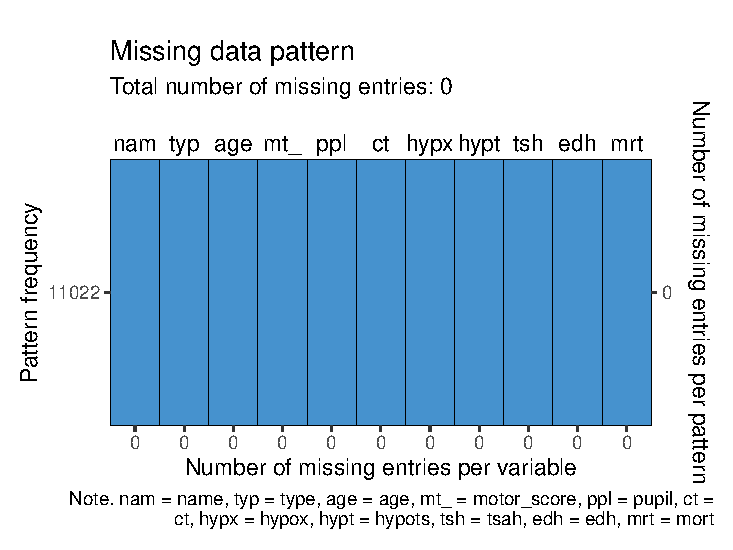
\includegraphics{Manuscript_files/figure-latex/impact-1} \end{center}

\end{CodeChunk}

-\textgreater{} Why are there no missings? According to the
\href{https://cran.r-project.org/web/packages/metamisc/metamisc.pdf}{vignette},
the data is already imputed (Steyerberg et al, 2008).

\begin{itemize}
\item
  MAR miss varying by cluster. Obs data patt differ per cluster. E.g.,
  in cluster 1 miss depends on age but not in cluster two. Split the
  dataframe and run \texttt{ampute()} on each cluster. -\textgreater{}
  TODO: also make MNAR missingness to heckman model. Maybe based on
  \texttt{ct} variable? Inclusion-selection variable. -\textgreater{}
  otherwise: use \texttt{leiden85} data on blood pressure with MNAR.
  Then run cox regression like the boshuizen article but with living
  situation as clusters. -\textgreater{} TODO: get analyses from
  \url{https://www.gerkovink.com/mimp/Contents/Exercises/Day\%203\%20-\%20Wednesday/Sensitivity_analysis/Sensitivity_analysis.html}.
\item
  ADD: \texttt{multilevel\_ampute()} wrapper function in \texttt{mice}.
\end{itemize}

\hypertarget{case-study-ii-popularity}{%
\subsection{Case Study II: Popularity}\label{case-study-ii-popularity}}

\begin{itemize}
\item
  What does the data look like? \texttt{popNCR} is a simulated dataset
  with pupils clustered in classes, \(n_{\text{participants}} = 2000\),
  \(n_{\text{clusters}} = 100\), on 7 variables:

  \begin{itemize}
  \tightlist
  \item
    \texttt{pupil} Pupil number within class,
  \item
    \texttt{class} Class number,
  \item
    \texttt{extrav} Pupil extraversion,
  \item
    \texttt{sex} Pupil gender,
  \item
    \texttt{texp} Teacher experience (years),
  \item
    \texttt{popular} Pupil popularity,
  \item
    \texttt{popteach} Teacher popularity.
  \end{itemize}
\item
  What are the ICCs? For \texttt{popular} the ICC is 0.33. For
  \texttt{popteach} it is 0.31. It would be wise to use multilevel
  modeling.
\item
  What does the missingness look like? Induced MAR/MNAR missingness.
  Missing data pattern:
\end{itemize}

\begin{CodeChunk}


\begin{center}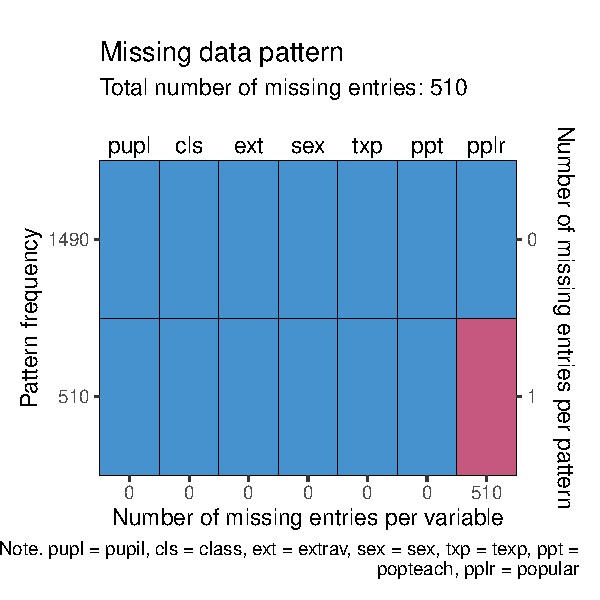
\includegraphics{Manuscript_files/figure-latex/pop_pat-1} \end{center}

\end{CodeChunk}

\begin{itemize}
\tightlist
\item
  Does the missing data of \texttt{popular} depend on \texttt{popteach}?
  Does the missingness in teacher popularity depend on pupil popularity?
  -\textgreater{} Check this by making a histogram of \texttt{popteach}
  separately for the pupils with known popularity and missing
  popularity, and the other way around.
\end{itemize}

\begin{CodeChunk}


\begin{center}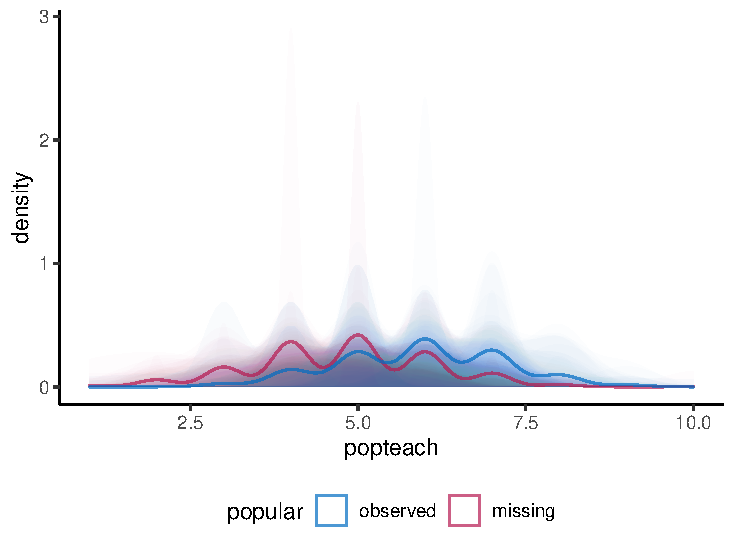
\includegraphics{Manuscript_files/figure-latex/pop_dist-1} \end{center}



\begin{center}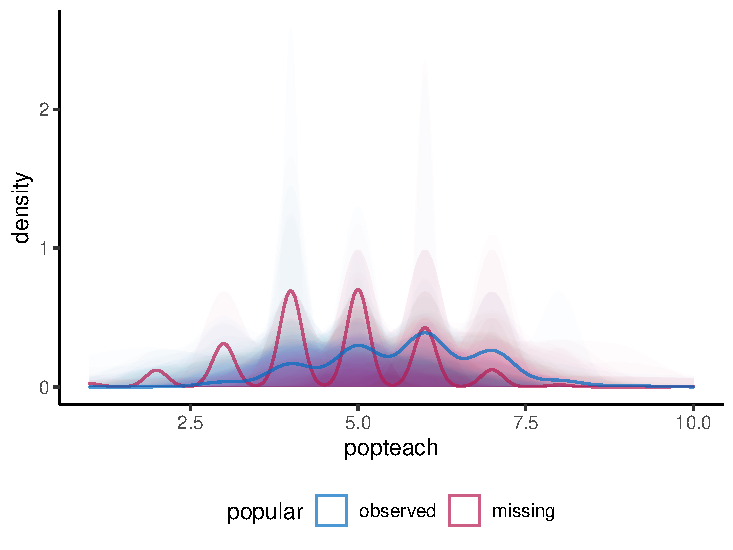
\includegraphics{Manuscript_files/figure-latex/pop_dist-2} \end{center}

\end{CodeChunk}

\begin{itemize}
\item
  We do see that the distribution for the missing \texttt{popular} is
  further to the right than the distribution for observed
  \texttt{popular}. This would indicate a right-tailed MAR missingness.
  In fact this is exactly what happens, because we created the
  missingness in these data ourselves. But we made it observable by
  examining the relations between the missingness in popular and the
  observed data in \texttt{popteach}. There is also a dependency between
  the missingness in teacher popularity and pupil popularity. The
  relation seems to be right-tailed as well.
\item
  We can impute the missingness the `standard' way, ignoring the
  multilevel structure of the data. This is surely invalid, given the
  high ICCs, but we'll do it anyways.
\item
  We'll use predictive mean matching to impute the continuous variables
  (some appear to be somewhat ordinal), and logistic regression to
  impute the binary variable \texttt{sex}. We do not use the observation
  identifier \texttt{pupil} or cluster identifier \texttt{class} as
  predictors to impute other variables.
\end{itemize}

\begin{CodeChunk}
\begin{CodeInput}
R> # dry run to get imputation parameters
R> ini <- mice(pop, maxit = 0)
R> 
R> # extract predictor matrix and adjust
R> pred <- ini$pred
R> pred[, c("class", "pupil")] <- 0
R> pred 
\end{CodeInput}
\begin{CodeOutput}
         pupil class extrav sex texp popular popteach school
pupil        0     0      1   1    1       1        1      1
class        0     0      1   1    1       1        1      1
extrav       0     0      0   1    1       1        1      1
sex          0     0      1   0    1       1        1      1
texp         0     0      1   1    0       1        1      1
popular      0     0      1   1    1       0        1      1
popteach     0     0      1   1    1       1        0      1
school       0     0      1   1    1       1        1      0
\end{CodeOutput}
\begin{CodeInput}
R> # impute the data, ignoring the cluster structure
R> imp_ignored <- mice(pop, maxit = 10, pred = pred, print = FALSE)
R> 
R> # check convergence of the imputation model
R> plot(imp_ignored)
\end{CodeInput}


\begin{center}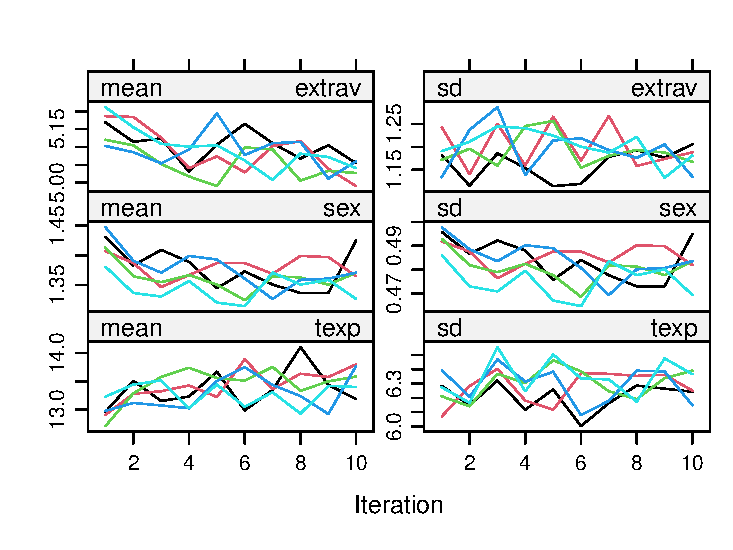
\includegraphics{Manuscript_files/figure-latex/pop-ignored-1} \end{center}



\begin{center}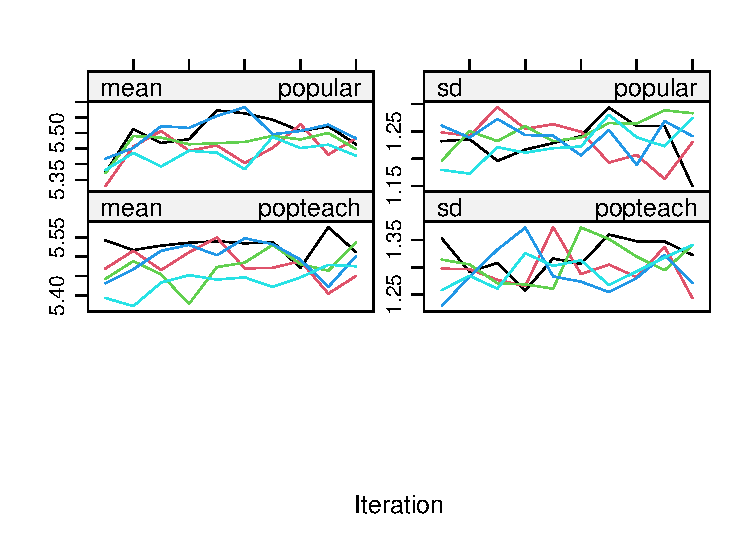
\includegraphics{Manuscript_files/figure-latex/pop-ignored-2} \end{center}

\begin{CodeInput}
R> # compare descriptives before and after imputation
R> psych::describe(pop)[, c("n", "mean", "median", "min", "max", "sd")]
\end{CodeInput}
\begin{CodeOutput}
            n  mean median min   max    sd
pupil    2000 10.65   11.0   1  26.0  5.97
class*   2000 50.37   51.0   1 100.0 29.08
extrav   1484  5.31    5.0   1  10.0  1.29
sex*     1504  1.56    2.0   1   2.0  0.50
texp     1024 11.80   12.0   2  25.0  6.26
popular  1490  4.83    4.8   0   9.1  1.34
popteach 1472  4.83    5.0   1  10.0  1.36
school   2000  5.54    6.0   1  10.0  2.89
\end{CodeOutput}
\begin{CodeInput}
R> psych::describe(mice::complete(imp_ignored))[, c("n", "mean", "median", "min", "max", "sd")] #note that this is just 1 imputation, not the pooled results
\end{CodeInput}
\begin{CodeOutput}
            n  mean median min   max    sd
pupil    2000 10.65     11   1  26.0  5.97
class*   2000 50.37     51   1 100.0 29.08
extrav   2000  5.25      5   1  10.0  1.27
sex*     2000  1.53      2   1   2.0  0.50
texp     2000 12.48     12   2  25.0  6.29
popular  2000  4.99      5   0   9.1  1.35
popteach 2000  5.02      5   1  10.0  1.39
school   2000  5.54      6   1  10.0  2.89
\end{CodeOutput}
\begin{CodeInput}
R> # TODO: add stripplot with boxplot overlay instead of the tables (make pooled one thick on top)
R> # TODO: pool mean median and sd
R> # feedback Stef: numbers, continuous statistics such as means, and uncertainty estimates. So we can pool the sd's. And leave out the min and max, because those are not normally distr.
R> # TODO: add FMI for each of the estimates? at least for the mean
R> 
R> # further inspection of the imputations
R> densityplot(imp_ignored)
\end{CodeInput}


\begin{center}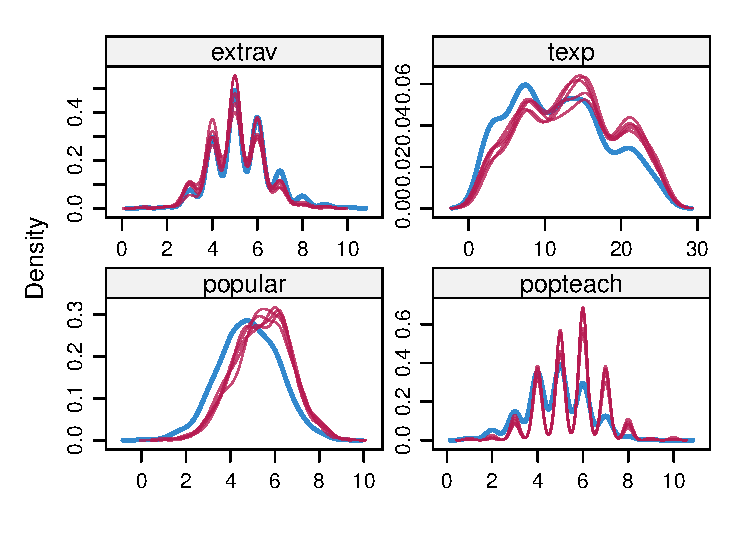
\includegraphics{Manuscript_files/figure-latex/pop-ignored-3} \end{center}

\begin{CodeInput}
R> # compare ICCs before and after imputation
R> ICCs <- data.frame(
+   vars = c("popular", "popteach", "texp"), 
+   incomplete = c(multilevel::ICC1(aov(popular ~ class, pop)), 
+                multilevel::ICC1(aov(popteach ~ class, pop)),
+                multilevel::ICC1(aov(texp ~ class, pop))), 
+   ignored = c(multilevel::ICC1(aov(popular ~ class, complete(imp_ignored))), 
+               multilevel::ICC1(aov(popteach ~ class, complete(imp_ignored))), 
+               multilevel::ICC1(aov(texp ~ class, complete(imp_ignored))))
+   )
R> ICCs
\end{CodeInput}
\begin{CodeOutput}
      vars incomplete   ignored
1  popular  0.3280070 0.2716802
2 popteach  0.3138658 0.2528468
3     texp  1.0000000 0.4395296
\end{CodeOutput}
\end{CodeChunk}

\begin{itemize}
\item
  As the original ICCs show, 100\% of the variance in \texttt{texp} can
  be attributed to the clustering variable \texttt{class}. This tells us
  that the multilevel structure of the data should be taken into
  account. If we don't, we'll end up with incorrect imputations, biasing
  the effect of the clusters towards zero.
\item
  We can also observe that the teacher experience increases slightly
  after imputation. This is due to the MNAR missingness in
  \texttt{texp}. Higher values for \texttt{texp} have a larger
  probability to be missing. This may not a problem, however, if at
  least one pupil in each class has teacher experience recorded, we can
  deductively impute the correct (i.e.~true) value for every pupil in
  the class.
\item
  We'll now use \texttt{class} as a predictor to impute all other
  variables.
\end{itemize}

\begin{CodeChunk}
\begin{CodeInput}
R> # adjust the predictor matrix
R> pred <- ini$pred 
R> pred[, "pupil"] <- 0
R> pred
\end{CodeInput}
\begin{CodeOutput}
         pupil class extrav sex texp popular popteach school
pupil        0     1      1   1    1       1        1      1
class        0     0      1   1    1       1        1      1
extrav       0     1      0   1    1       1        1      1
sex          0     1      1   0    1       1        1      1
texp         0     1      1   1    0       1        1      1
popular      0     1      1   1    1       0        1      1
popteach     0     1      1   1    1       1        0      1
school       0     1      1   1    1       1        1      0
\end{CodeOutput}
\begin{CodeInput}
R> # impute the data, cluster as predictor
R> imp_predictor <- mice(pop, maxit = 10, pred = pred, print = FALSE)
\end{CodeInput}
\begin{CodeOutput}
Warning: Number of logged events: 325
\end{CodeOutput}
\begin{CodeInput}
R> # check logged events
R> head(imp_predictor$loggedEvents)
\end{CodeInput}
\begin{CodeOutput}
  it im      dep   meth
1  1  1   extrav    pmm
2  1  1      sex logreg
3  1  1     texp    pmm
4  1  1  popular    pmm
5  1  1 popteach    pmm
6  1  1 popteach    pmm
                                                                                                                                                                                                                                                       out
1                                                                                                                                                                                                                                                   school
2                                                                                                                                                                                                                                                   school
3                                                                                                                                                                                                                                                   school
4                                                                                                                                                                                                                                             texp, school
5                                                                                                                                                                                                                                                     texp
6 mice detected that your data are (nearly) multi-collinear.\nIt applied a ridge penalty to continue calculations, but the results can be unstable.\nDoes your dataset contain duplicates, linear transformation, or factors with unique respondent names?
\end{CodeOutput}
\begin{CodeInput}
R> ## "The mice() function detects multicollinearity, and solves the problem by removing one or more predictors for the model", in this case texp is removed as predictor of popular and popteach.
R> 
R> # check convergence of the imputation model
R> plot(imp_predictor)
\end{CodeInput}


\begin{center}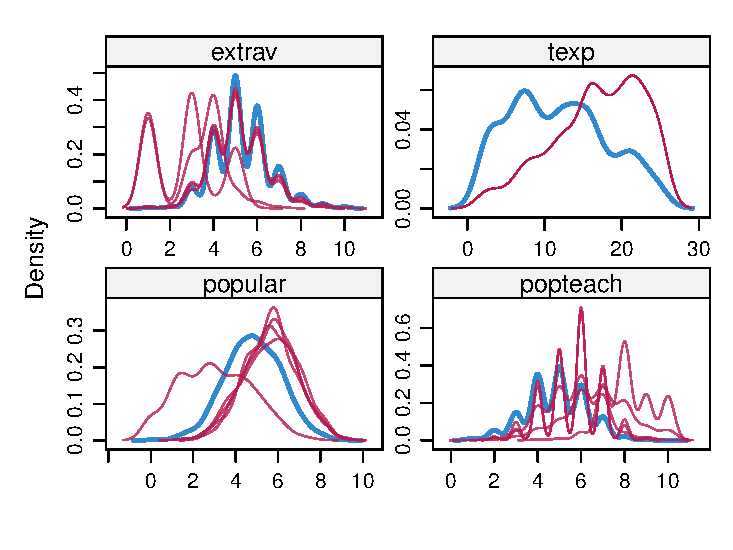
\includegraphics{Manuscript_files/figure-latex/pop-predictor-1} \end{center}



\begin{center}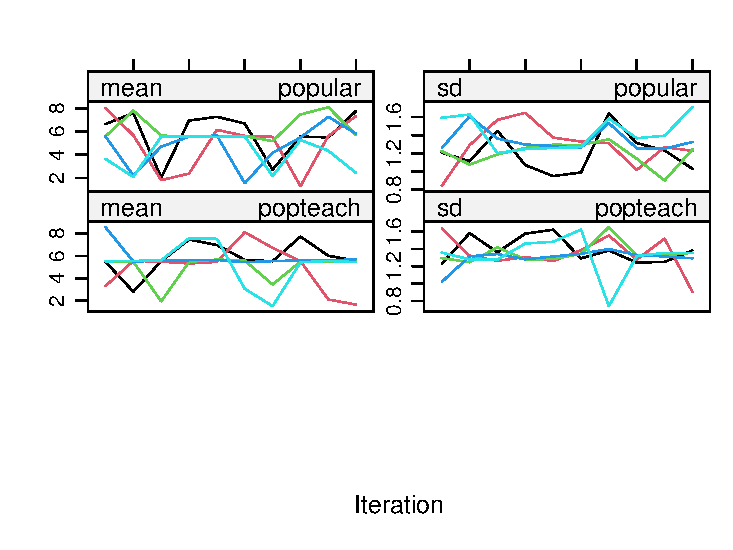
\includegraphics{Manuscript_files/figure-latex/pop-predictor-2} \end{center}

\begin{CodeInput}
R> # compare descriptives before and after imputation
R> psych::describe(pop)[, c("n", "mean", "median", "min", "max", "sd")]
\end{CodeInput}
\begin{CodeOutput}
            n  mean median min   max    sd
pupil    2000 10.65   11.0   1  26.0  5.97
class*   2000 50.37   51.0   1 100.0 29.08
extrav   1484  5.31    5.0   1  10.0  1.29
sex*     1504  1.56    2.0   1   2.0  0.50
texp     1024 11.80   12.0   2  25.0  6.26
popular  1490  4.83    4.8   0   9.1  1.34
popteach 1472  4.83    5.0   1  10.0  1.36
school   2000  5.54    6.0   1  10.0  2.89
\end{CodeOutput}
\begin{CodeInput}
R> psych::describe(mice::complete(imp_predictor))[, c("n", "mean", "median", "min", "max", "sd")] #note that this is just 1 imputation, not the pooled results
\end{CodeInput}
\begin{CodeOutput}
            n  mean median min   max    sd
pupil    2000 10.65     11   1  26.0  5.97
class*   2000 50.37     51   1 100.0 29.08
extrav   2000  6.20      6   1  10.0  2.00
sex*     2000  1.52      2   1   2.0  0.50
texp     2000 14.26     15   2  25.0  6.55
popular  2000  5.03      5   0   9.1  1.35
popteach 2000  5.03      5   1  10.0  1.38
school   2000  5.54      6   1  10.0  2.89
\end{CodeOutput}
\begin{CodeInput}
R> # further inspection of the imputations
R> densityplot(imp_predictor)
\end{CodeInput}


\begin{center}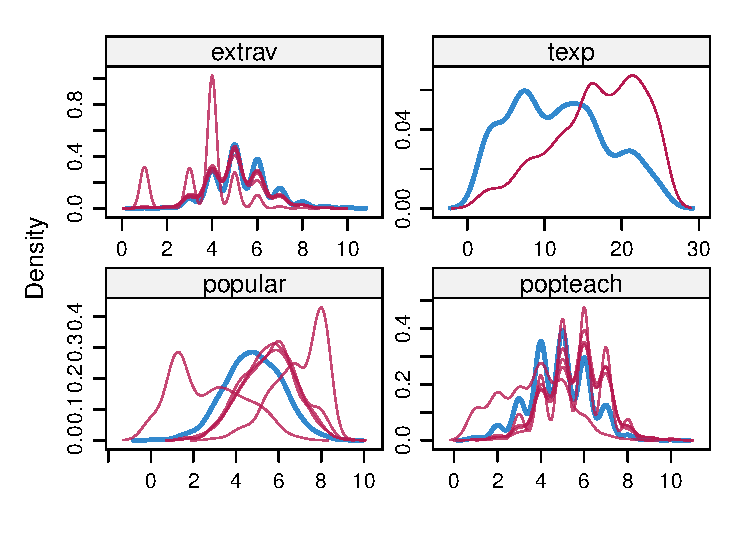
\includegraphics{Manuscript_files/figure-latex/pop-predictor-3} \end{center}

\begin{CodeInput}
R> # compare ICCs before and after imputation
R> ICCs <- ICCs %>% cbind(
+            predictor = c(multilevel::ICC1(aov(popular ~ class, complete(imp_predictor))), 
+                         multilevel::ICC1(aov(popteach ~ class, complete(imp_predictor))), 
+                         multilevel::ICC1(aov(texp ~ class, complete(imp_predictor))))
+            )
R> ICCs
\end{CodeInput}
\begin{CodeOutput}
      vars incomplete   ignored predictor
1  popular  0.3280070 0.2716802 0.3550567
2 popteach  0.3138658 0.2528468 0.3306035
3     texp  1.0000000 0.4395296 1.0000000
\end{CodeOutput}
\end{CodeChunk}

\begin{itemize}
\item
  Now, we can clearly see that the imputed values of \texttt{texp} are
  higher than the observed values, which is in line with right-tailed
  MNAR.
\item
  The ICCs are way more in line with the ICCs in the incomplete data.
  But this is a quick and dirty way of imputing multilevel data. We
  \emph{should} be using a multilevel model.
\end{itemize}

\hypertarget{amputation}{%
\subsection{Amputation}\label{amputation}}

\begin{itemize}
\tightlist
\item
\end{itemize}

\hypertarget{modeling-choices}{%
\subsection{Modeling choices}\label{modeling-choices}}

\begin{itemize}
\item
  Which models will we discuss? We'll build the model to grow in
  complexity. The final model is the most complex but also the most
  versatile.
\item
  Note on model complexity: Typically, we should at least use random
  intercepts, but often random slopes as well. Ideally we impute with
  random everything and heteroscedastic errors: most generic method (no
  worry about congeniality, but don't mention the term) -\textgreater{}
  Refer to other papers for background, we'll focus just on the software
  implementation of the situations mentioned there. Sometimes there's
  little reason to assume some variable is affected by heterogeneity.
  -\textgreater{} Refer to \citet{meng94}, an Audigier paper, and a
  paper by Grund on congeniality and random slopes.
\item
  Step 0: As predictor + CCA to scare off users
\item
  Step 1: Random intercepts
\item
  Step 2: Random slopes
\item
  Step 3: Residuals
\item
  Heckman model for MNAR
\item
  What do the different implementations look like? How to define the
  imputation model(s) in \texttt{mice}?
\end{itemize}

\hypertarget{step-0}{%
\subsection{Step 0}\label{step-0}}

\begin{itemize}
\item
  AKA multilevel imputation for dummies.
\item
  Doesn't work for systematic missingness.
\end{itemize}

\hypertarget{step-1-3-mnar}{%
\subsection{Step 1-3 + MNAR}\label{step-1-3-mnar}}

\begin{itemize}
\tightlist
\item
  TODO: fill in.
\end{itemize}

\hypertarget{pooling}{%
\subsection{Pooling}\label{pooling}}

\begin{itemize}
\item
  Analysis of scientific interest.
\item
  Pooling using \texttt{mitml}.
\item
  Pooling `regular' parameters vs more `exotic' parameters (SE of
  residual errors, or autocorrelation)
\item
  ADD: export \texttt{mids} objects to other packages like \texttt{lme4}
  or \texttt{coxme}?
\end{itemize}

\hypertarget{discussion}{%
\section{Discussion}\label{discussion}}

\begin{itemize}
\item
  JOMO in \texttt{mice} --\textgreater{} on the side for now
\item
  Additional levels of clustering
\item
  More complex data types: timeseries and polynomial relationship in the
  clustering.
\end{itemize}

\renewcommand\refname{References}
\bibliography{../References/multilevelmice.bib}


\end{document}
